



\documentclass[journal]{IEEEtran}
\hyphenation{op-tical net-works semi-conduc-tor}
%%%%%%%%%%%%%%%%%%%%%%%%%%%%%%%%%%%%%%%%%%%%%%%%%%%%%%%%%%%%%%%%%%
%%%%%%%%%%%%%%%%%%%%%%%%%%%%%%%%%%%%%%%%%%%%%%%%%%%%%%%%%%%%%%%%%%
%%%%%%%%%%%%%%%%%%%%%%%%% PACKAGES %%%%%%%%%%%%%%%%%%%%%%%%%%%%%%%
%%%%%%%%%%%%%%%%%%%%%%%%%%%%%%%%%%%%%%%%%%%%%%%%%%%%%%%%%%%%%%%%%%
%%%%%%%%%%%%%%%%%%%%%%%%%%%%%%%%%%%%%%%%%%%%%%%%%%%%%%%%%%%%%%%%%%
\usepackage[T1]{fontenc}
\usepackage[utf8]{inputenc}
\usepackage{lmodern}
\usepackage[portuguese]{babel}
\usepackage{graphicx}
\usepackage{fancyhdr}
\usepackage{caption}
\usepackage{subcaption}
\usepackage{placeins}
\pagestyle{fancy}
\usepackage{color}
\usepackage{cancel}
\newcommand{\HRule}{\rule{\linewidth}{0.5mm}}
\usepackage{steinmetz}
\graphicspath{{../images/}}

\begin{document}

\title{Experimento 5: Análise no Domínio da Frequência}

\author{  \begin{tabular}{llr} \
    & & \\[0.05cm]
    Professor: & Henrique Cezar Ferreira & \\
    Alunos:& & \\
    & Juarez A.S.F                        & 11/0032829\\
    & Luís Henrique Vieira Amaral           & 10/0130488  
      \end{tabular}
      }


\maketitle

%@@@@@@@@@@@@@@@@@@@@@@@@@@@@@@@@@@@@@@@@@@@
%@@@@@@@@@@@@@@@@      OBJETIVOS      @@@@@@@@@@@@@@@@@@
%@@@@@@@@@@@@@@@@@@@@@@@@@@@@@@@@@@@@@@@@@@@
\section{Objetivos}
Obter experimentalmente o diagrama de Bode para a 
magnitude e fase da planta servo angular Quanser.
%@@@@@@@@@@@@@@@@@@@@@@@@@@@@@@@@@@@@@@@@@@@@@
%@@@@@@@@@@@@@@        INTRODUÇÃO       @@@@@@@@@@@@@@@@@@@@ 
%@@@@@@@@@@@@@@@@@@@@@@@@@@@@@@@@@@@@@@@@@@@@@
\section{Introdução Teórica}

Consideramos para análise em frequência a seguinte função
 de transferência:

\begin{equation}
  H(s) = \frac{K}{\tau s + 1}
  \label{eq:FT}
\end{equation}

substituindo $\tau$ por $jw$, onde w é a frequência em
rad/s, obtemos:

\begin{equation}
  H(jw) = \frac{K}{1 +  (w \tau)j }
\end{equation}

de onde temos o módulo e a fase:
\begin{equation}
  \left\{
  \begin{array}{l}
    |H(jw)| = \frac{|K|}{\sqrt{(1 +  (w \tau)^2)} } \\
    \phase{H(jw)} = -\tan ^{-1} {(w \tau)}
  \end{array}
  \right.
\end{equation}

tirando 20 vezes o logaritmo na base dez do módulo, obtemos:

\begin{equation}
  20 \log |H(jw)| = 20 \log |K| - 20 \log (\sqrt{(1 +  (w \tau)^2)} )
\end{equation}

dividimos então a análise em duas etapas:
\begin{itemize}
\item para altas frequências $\sqrt{(1 +  (w \tau)^2)}  \approx |w \tau|$
\item para baixas frequências $\sqrt{(1 +  (w \tau)^2)}  \approx 1$
\end{itemize}

portanto:

\begin{equation}
\left\{
\begin{array}{l}
  20 \log |H(jw)| \approx 20 \log |K/\tau| - 20 \log w , \mbox{ w $\gg$ $\frac{1}{\tau}$} \\
20 \log |H(jw)| \approx 20 \log |K/\tau|, \mbox{ w $\ll$ $\frac{1}{\tau}$} \\
20 \log |H(jw)| = 20 \log |K/\tau| - 20 \log \sqrt 2, \mbox{ w = $\frac{1}{\tau}$} \\
\end{array}
\right.
\label{eq:mod}
\end{equation}

para a frequência obtemos:

\begin{equation}
\left\{
\begin{array}{l}
\phase{H(jw)} \approx -90º, \mbox{ w $\gg$ $\frac{1}{\tau}$} \\
\phase{H(jw)} \approx 0º, \mbox{ w $\ll$ $\frac{1}{\tau}$} \\
\phase{H(jw)} = -45º, \mbox{ w = $\frac{1}{\tau}$} \\
\end{array}
\right.
\label{eq:phase}
\end{equation}

Ao plotarmos o logaritmo da frequência pelo módulo e pela fase
se H(jw) obtemos os diagramas de Bode. A facilidade dessa análise
consiste em, por meio da aproximação por assíntotas, dividir a
resposta em frequência como a soma das respostas para cada polo e
zero da função de transferência.

%@@@@@@@@@@@@@@@@@@@@@@@@@@@@@@@@@@@@@@@@@@@
%@@@@@@@@@@@@       PROCEDIMENTOS        @@@@@@@@@@@@@@@@@@
%@@@@@@@@@@@@@@@@@@@@@@@@@@@@@@@@@@@@@@@@@@@
\section{Descrição Experimental}
\begin{itemize}
 \item Primeiramente, o modelo bode\_IP02.mdl que continha o 
subsistema real do IP02  e outro subsistema teórico foi aberto no 
Simulink. Na entrada havia uma senóide  com fase nula e amplitude e 
frequências ajustáveis. Abriu-se o script setup\_lab\_IP02\_bode.m 
que carregava todos os parâmetros e variáveis do diagrama.

\item Após executar o script bode\_plot.m verificou-se se a 
aproximação assintótica calculada no pré-relatório se assemelhava com 
o diagrama obtido experimentalmente.

\item A partir dos valores de frequência e amplitude da tabela dada, 
os valores de amplitude (dB) e fase (graus) foram obtidos. Para a 
obtenção destes dados, o programa amp\_fase.m foi executado.

\item Por fim, os pontos obtidos na tabela foram plotados nos 
diagramas de Bode teóricos para que fossem feitas as comparações. Os 
pontos foram plotados a partir dos comandos especificados no roteiro 
do experimento: subplot(2,1,1); semilogx(w,M,’o’); hold on; e 
subplot(2,1,2); semilogx(w, phi,’o’); hold on; para amplitude e fase 
respectivamente.
\end{itemize}

%@@@@@@@@@@@@@@@@@@@@@@@@@@@@@@@@@@@@@@@@@@@@@@@@
%@@@@@@@@@@@@@@@@@@@       DADOS      @@@@@@@@@@@
%@@@@@@@@@@@@@@@@@@@@@@@@@@@@@@@@@@@@@@@@@@@@@@@@
\section{Resultados}
A tabela a seguir mostra os dados experimentais:
\FloatBarrier
\begin{table}[!htp]
 \centering
 \begin{tabular}{|l|l|l|}\hline
 Frequencia(rad/seg) &         Amplitude M (dB) &      Fase(Graus) \\ 
\hline 
 		 1 &  5.2556 &  1.1495 \\ \hline 
		 2 &  3.3802 &  -2.9835 \\ \hline 
		 3 &  4.1187 &  -4.6712 \\ \hline 
		 4 &  4.9935 &  -7.2857 \\ \hline 
		 5 &  4.9383 &  -8.9341 \\ \hline 
		 6 &  4.8837 &  -9.7783 \\ \hline 
		 7 &  4.8689 &  -10.9161 \\ \hline 
		 10 &  4.6464 &  -16.4334 \\ \hline 
		 15 &  4.2467 &  -23.3527 \\ \hline 
		 20 &  3.7984 &  -29.9879 \\ \hline 
		 30 &  2.6781 &  -41.6042 \\ \hline 
		 40 &  1.5014 &  -49.7234 \\ \hline 
		 60 &  -0.6492 &  -59.8260 \\ \hline 
		 80 &  -2.5478 &  -68.0906 \\ \hline 
		 100 &  -4.1486 &  -73.2130 \\ \hline 
		 100 &  -4.1486 &  -73.2130 \\ \hline 
 \end{tabular}
  \caption{dados experimentais}
\end{table}
\FloatBarrier

O gráfico obtido é mostrado a seguir:
\FloatBarrier
\begin{figure}[!htp]
   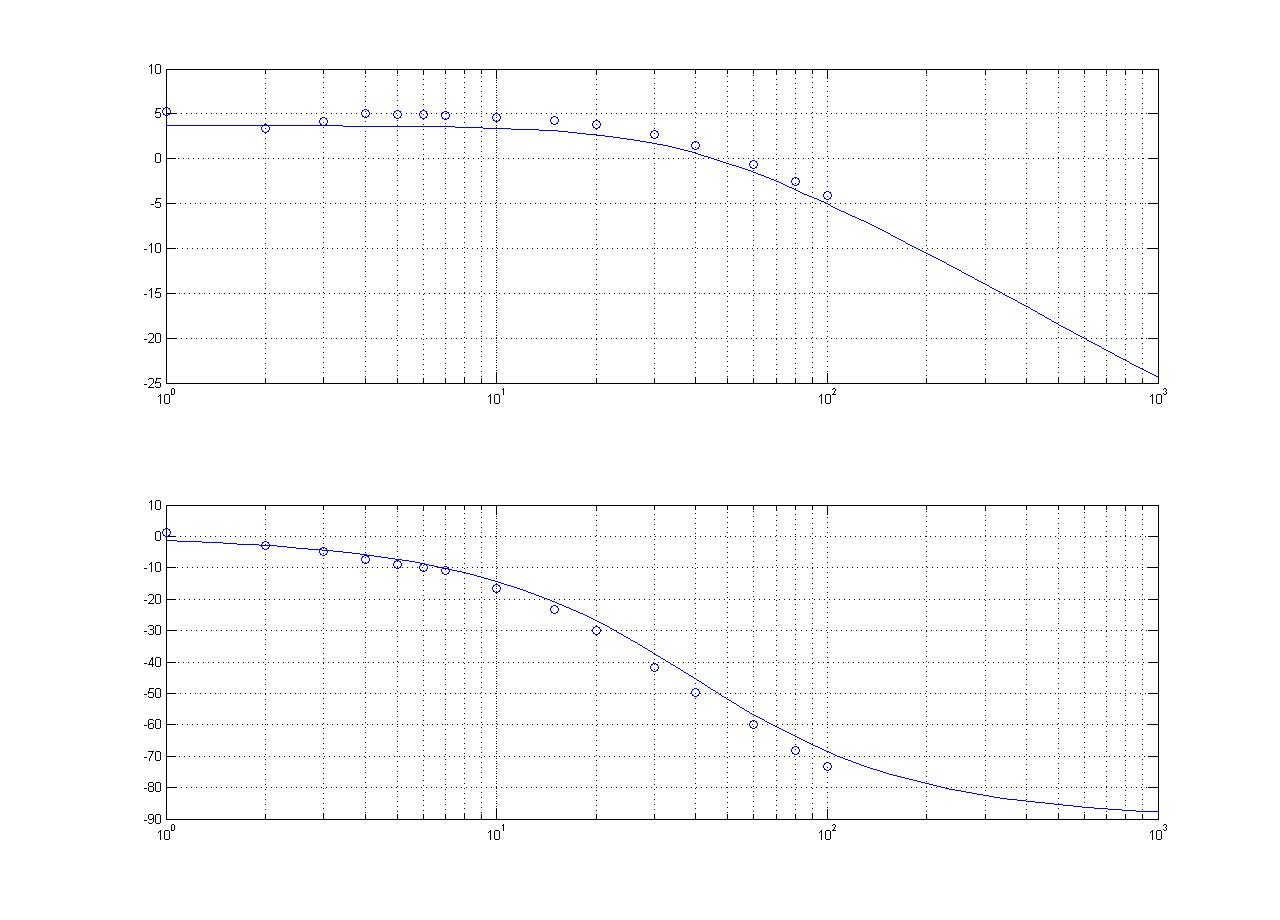
\includegraphics[scale=0.2]{../images/exp5_plot.jpg}
    \caption{resposta em frequência da planta angular Quanser}
    \label{fig:step}
\end{figure}
\FloatBarrier

Em ambos os gráficos temos o no eixo x o logaritmo da frequência,
já no eixo y temos o módulo da resposta no gráfico de cima e a fase
no gráfico de baixo. A linha contínua foi obtida usando a função freqs()
sob a função de transferência na fórmula \ref{eq:FT} com os 
parâmetros K = 1.5286 e $\tau = 0.0254$
e os círculos são
os pontos experimentais obtidos para algumas frequências de entrada.
%@@@@@@@@@@@@@@@@@@@@@@@@@@@@@@@@@@@@@@@@@@@
%@@@@@@@@@@@@@@       Análise         @@@@@@@@@@@@@@@@@@@@@@
%@@@@@@@@@@@@@@@@@@@@@@@@@@@@@@@@@@@@@@@@@@@@
\section{Discussão}

Notamos que a aproximação da previsão teórica com os dados 
experimentais é
satisfatória, pequenas diferenças,no entanto, são observáveis. No 
gráficos para a amplitude os pontos estão de forma geral acima da
curva teórica, enquanto no gráfico da fase eles estão a baixo.
Como pode ser visto pela fórmula \ref{eq:mod}, a fase  de -45º 
é atingida na frequência $\frac{1}{\tau}$.Esse valor de fase foi
obtido experimentalmente mais para a esquerda do que a previsão 
teórica. Isso nos sugere que o valor real de $\frac{1}{\tau}$ seja 
menor que aquele utilizado, o que implica um valor de $\tau > 0.0254$.
Da mesma forma, a amplitude em baixas frequências depende do fator 
$K/\tau$, como vemos em na fórmula \ref{eq:mod}. Como o experimental 
está acima do teórico, sabemos que a razão $K/\tau$ real é maior que 
a utilizada, juntando essa informação
com a análise anterior, vemos que o valor real de K deve ser maior que
1.5286.

Outra análise que poderia ser feita sobre os dados experimentais seria
determinar a forma função de transferência e seus parâmetros. Caso 
não soubéssemos a fórmula da função de transferência a forma da 
resposta
experimental nos daria uma ideia de que a função de 
transferência deve ter a forma $\frac{A}{1 + s/w_0}$, isto porque:
\begin{itemize}
 \item a queda de -20db para altas frequência nos indica a presença 
de um polo simples
  \item o valor do ganho diferente de zero para baixas frequências
  indica a constante A no numerador.
\end{itemize}

Além disso, uma vez que temos uma previsão para a função de 
transferência, podemos estimar os valores pela análise do gráfico.
Supondo uma função na forma $\frac{A}{1 + s/w_0}$, podemos determinar:
\begin{itemize}
 \item $w_0$ ao determinar a frequência de -3db
 \item K ao medir o ganho em baixas frequências.
\end{itemize}


Fora essa pequena diferença encontrada entre os dados experimentais e 
a previsão teórica, o experimento foi feito sem maiores dificuldades.

%@@@@@@@@@@@@@@@@@@@@@@@@@@@@@@@@@@@@@@@@@@@@@
%@@@@@@@@@@@@@@       Conclusão         @@@@@@@@@@@@@@@@@@@@@@
%@@@@@@@@@@@@@@@@@@@@@@@@@@@@@@@@@@@@@@@@@@@@@

\section{Conclusão}
O experimento permitiu estudar a  resposta em frequência para a 
planta Quanser angular e comparar os resultados experimentais
com aqueles esperados teoricamente. Os resultados obtidos
estiveram de bom acordo com a teoria e as pequenas diferenças
observadas nos deram um ideia de como melhorar a estimativa dos 
parâmetros da real função de transferência.
%@@@@@@@@@@@@@@@@@@@@@@@@@@@@@@@@@@@@@@@@@@@@@@
%@@@@@@@@@@@@@@       REFERÊNCIAS     @@@@@@@@@@@@@@@@@@@@@@
%@@@@@@@@@@@@@@@@@@@@@@@@@@@@@@@@@@@@@@@@@@@@@@
\begin{thebibliography}{9}    
   \bibitem{ADL-NISE}
      Nise, N.S.
      \emph{Engenharia de Sistemas de Controle}
     5ª ed.
    LTC, 2009.

   \bibitem{ADL-OGATA}
      Ogata, K.
      \emph{Moder Control Engeeniring}
     5ª ed.
    Pearson, 2010.
   
\end{thebibliography}
\end{document}


